\documentclass{article}
\usepackage{tikz}

\begin{document}

\section{The Existence of Derivatives:}
A function $f$ is said to be differentiable at $x=a$ if $f'(a)$ exists. At points where $f$ is not differentiable, we say that the derivative does not exist. Common ways for a derivative to not exist are shown.

\begin{figure}[h]
\centering
\begin{minipage}[b]{0.5\textwidth}
\centering
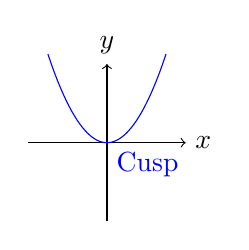
\begin{tikzpicture}[scale=0.5]
  % Cusp
  \draw[->] (-2,0) -- (2,0) node[right] {$x$};
  \draw[->] (0,-2) -- (0,2) node[above] {$y$};
  \draw[domain=-1.5:1.5, smooth, variable=\x, blue] plot ({\x}, {\x*\x});
  \node[below right, blue] at (0,0) {Cusp};
\end{tikzpicture}
\end{minipage}%
\begin{minipage}[b]{0.5\textwidth}
\centering
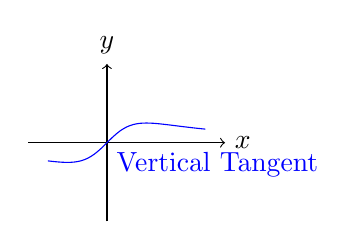
\begin{tikzpicture}[scale=0.5]
  % Vertical tangent
  \draw[->] (-2,0) -- (3,0) node[right] {$x$};
  \draw[->] (0,-2) -- (0,2) node[above] {$y$};
  \draw[domain=-1.5:2.5, smooth, variable=\x, blue] plot ({\x}, {\x/(1+\x*\x)});
  \node[below right, blue] at (0,0) {Vertical Tangent};
\end{tikzpicture}
\end{minipage}\\[20pt]
\begin{minipage}[b]{0.5\textwidth}
\centering
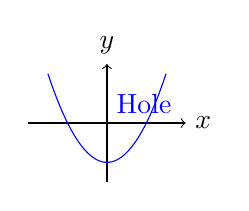
\begin{tikzpicture}[scale=0.5]
  % Hole
  \draw[->] (-2,0) -- (2,0) node[right] {$x$};
  \draw[->] (0,-1.5) -- (0,1.5) node[above] {$y$};
  \draw[domain=-1.5:1.5, smooth, variable=\x, blue] plot ({\x}, {(\x-1)*(\x+1)});
  \node[above right, blue] at (0,0) {Hole};
\end{tikzpicture}
\end{minipage}%
\begin{minipage}[b]{0.5\textwidth}
\centering
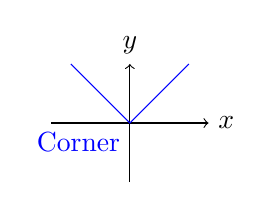
\begin{tikzpicture}[scale=0.5]
  % Corner
  \draw[->] (-2,0) -- (2,0) node[right] {$x$};
  \draw[->] (0,-1.5) -- (0,1.5) node[above] {$y$};
  \draw[domain=-1.5:1.5, variable=\x, blue] plot ({\x}, {abs(\x)});
  \node[below left, blue] at (0,0) {Corner};
\end{tikzpicture}
\end{minipage}
\caption{Different Types of Discontinuities}
\label{fig:discontinuities}
\end{figure}

\end{document}